\subsection{Общие сведения о нейронных сетях}
% todo what is nn
\subsubsection{Многослойный перцептрон}
Описанный Фрэнком Розенблаттом перцептрон -- это линейная модель классификации.
Она делит пространство входов нейронной сети на две части гиперплоскостью.

Перцептрон состоит из элементов трех видов: сенсорные, ассоциативные и
реагирующие. Сенсорные элементы вырабатывают сигнал под воздействием энергии.
Ассоциативные элементы выдают сигнал, когда алгебраическая сумма входящих
сигналов превышает пороговую величину $\theta > 0$. Реагирующий элемент выдает
сигнал $+1$, если сумма входных его сигналов строго положительна, и $-1$, если
сумма входных сигналов строго отрицательная.
\begin{figure}[h]
\centering
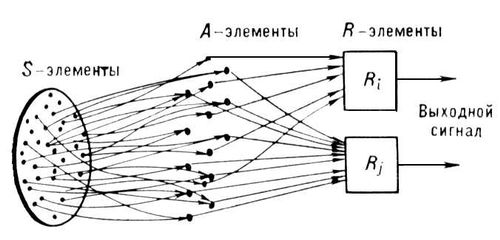
\includegraphics[width=0.5\textwidth]{Perceptron2}
\caption{Перцептрон. Источник: http://www.machinelearning.ru/wiki/index.php?title=Изображение:Perceptron2.jpg}
\label{fig:perceptron}
\end{figure}
\subsubsection{Сверточные нейронные сети}
Сверточные нейнонные сети часто применяются в задачах распознавания образов.
Главной составляющей СНС является слой свертки.

Основная идея сверточной сети -- обработка участка изображения независимо от
его положения. Слой свертки проходит <<окном>> по изображению и пытается
выделить признаки, строя их карту. Более строго этот процесс можно записать
с помощью формулы:
\[
y^{l}_{i, j} = \sum_{-d<=a,b<=d} W_{a,b}x^l_{i + a, j + b},
\]
где $y^l_{i, j}$ -- результат свертки на уровне $l$, а $x^l_{i, j}$ её вход (т.е.
выход предыдущего слоя), $W$ -- матрица весовых коэффициентов\cite{deeplearning}. 
На рисуноке \ref{fig:conv_calc} продемонстрирован пример подсчета результата по 
данной формуле.
\begin{figure}[h]
\centering
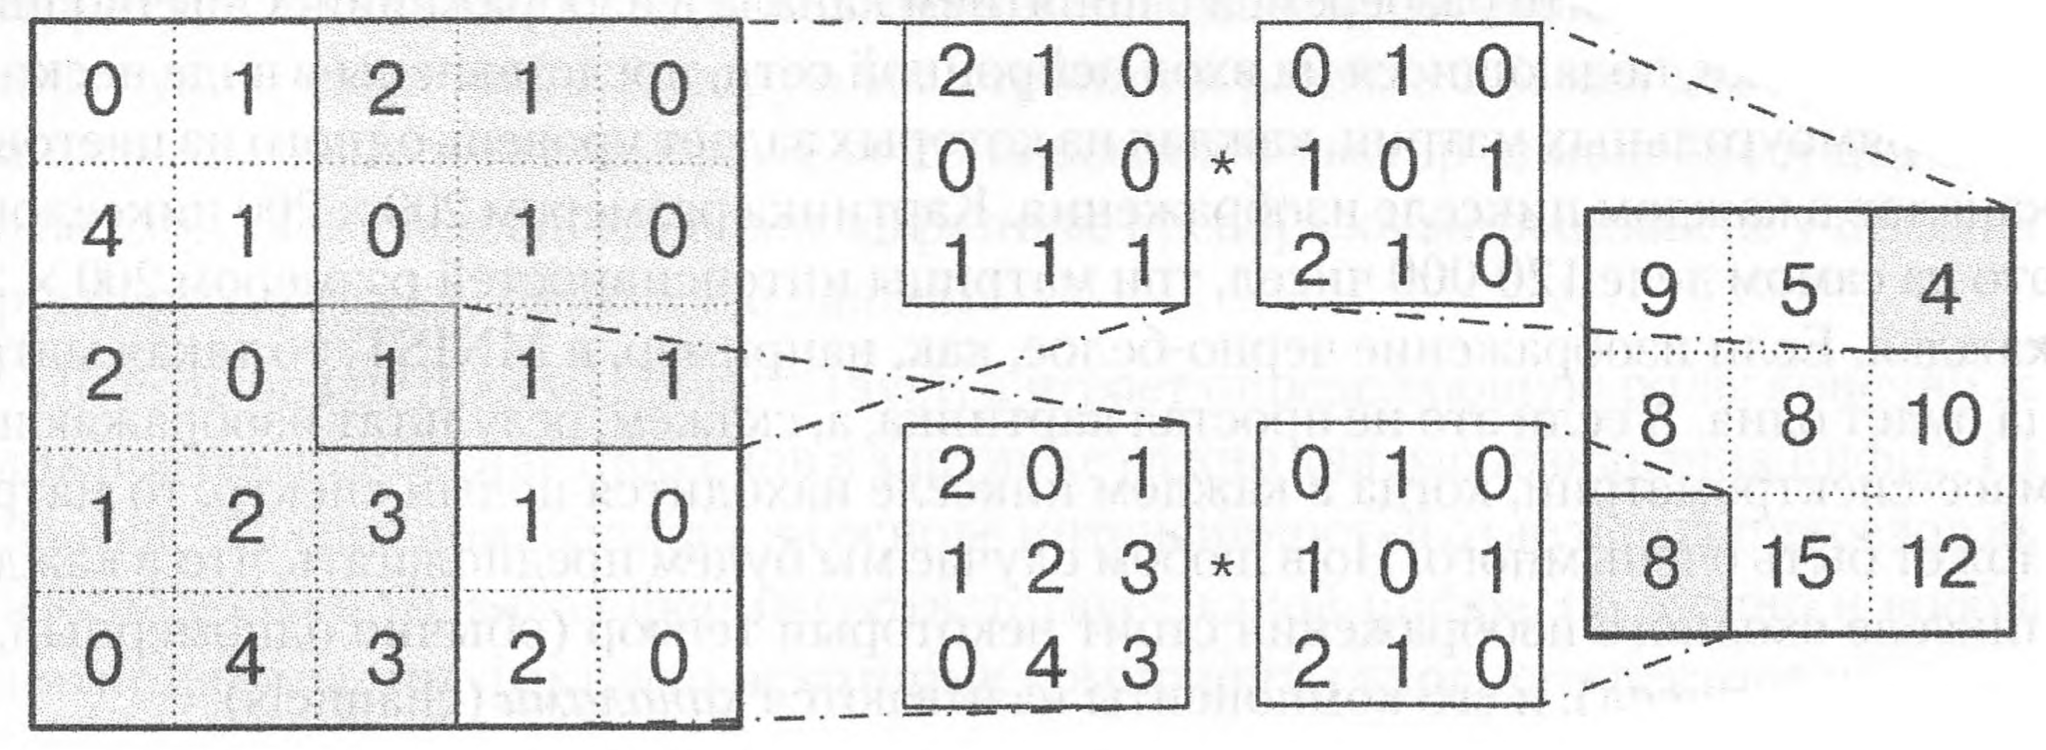
\includegraphics[width=0.8\textwidth]{conv_calc}
\caption{Пример подсчета результата свертки. Источник: \cite{deeplearning}}
\label{fig:conv_calc}
\end{figure}


% todo pooling
% todo LeNet
\subsubsection{Рекуррентные нейронные сети}
Часто исходными данными для нейронных сетей служат последовательности, имеющие
зависимости соседних точек друг от друга. Для выражения такой зависимости
применяются рекуррентные нейронные сети, где связи могут идти не только от
нижнего слоя к верхнему, но и от нейрона к самому себе. 

\begin{figure}[h]
\centering
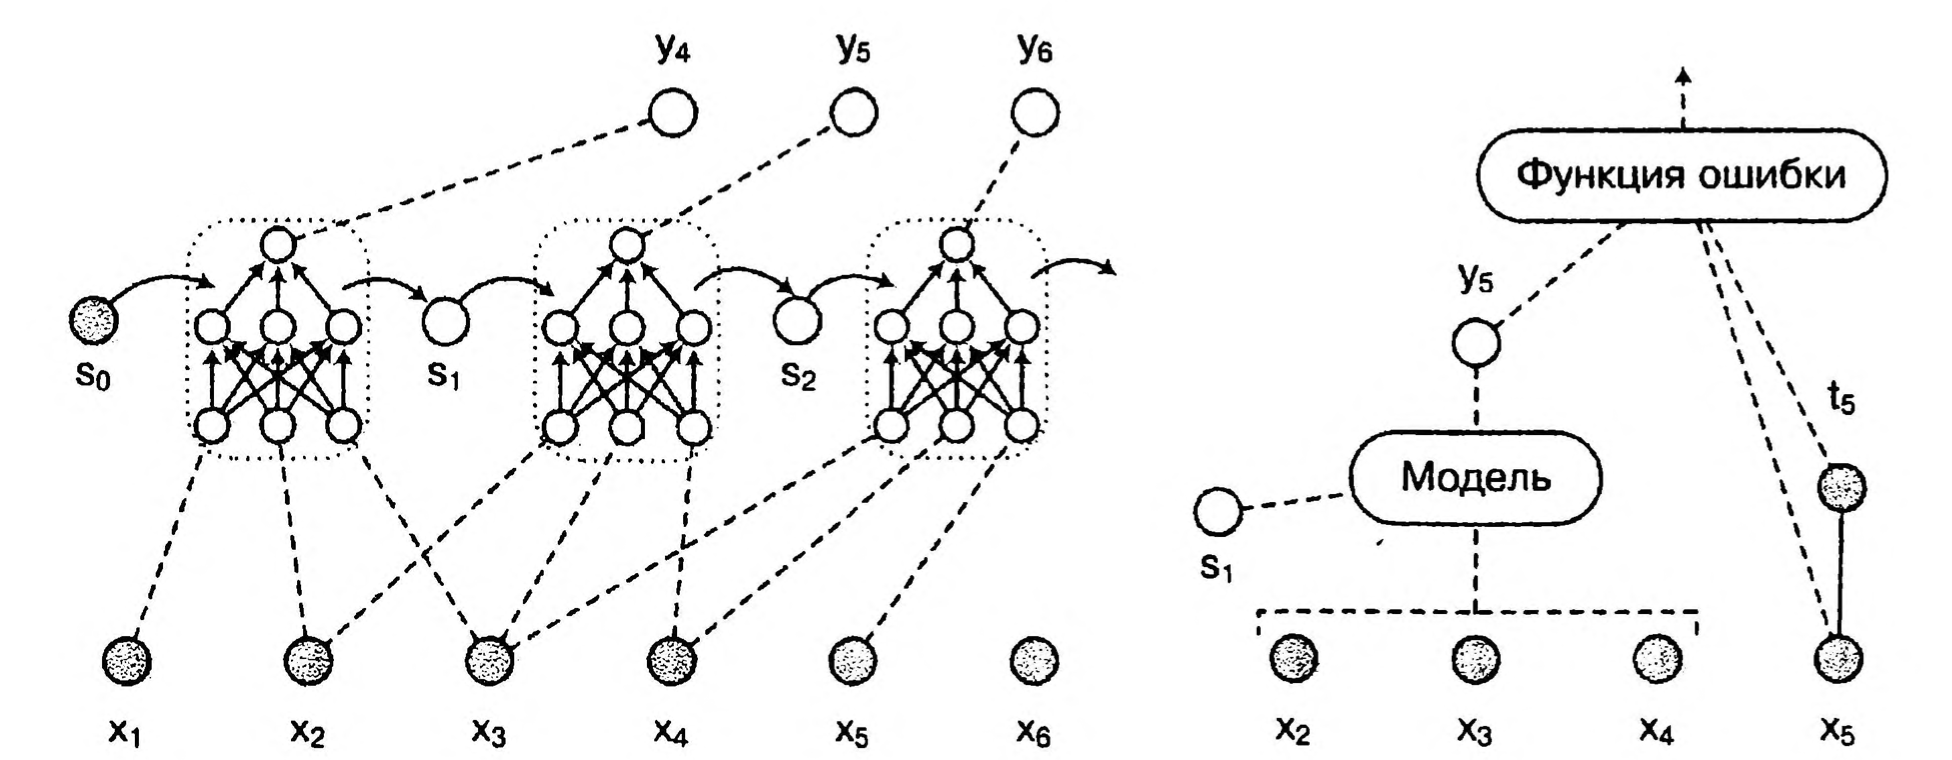
\includegraphics[width=0.8\textwidth]{recurrent_network}
\caption{Рекуррентная нейронная сеть. Источник: \cite{deeplearning}}
\label{fig:recurrent_network}
\end{figure}

На практике часто используется архитектура Long Short-Term Memory (LSTM). Она
состоит из трёх основных видов узлов (вентилей): входной, забывающий и выходной.
На вход ей подаются два вектора: вектор входных данных $x_t$ и вектор скрытого
состояния $h_{t-1}$. Внутри каждого блока есть векторы, выполняющий функцию
памяти (ячейка памяти)\cite{deeplearning}. Это демонстрирует схема на рис. \ref{fig:lstm}.
\begin{figure}[h]
\centering
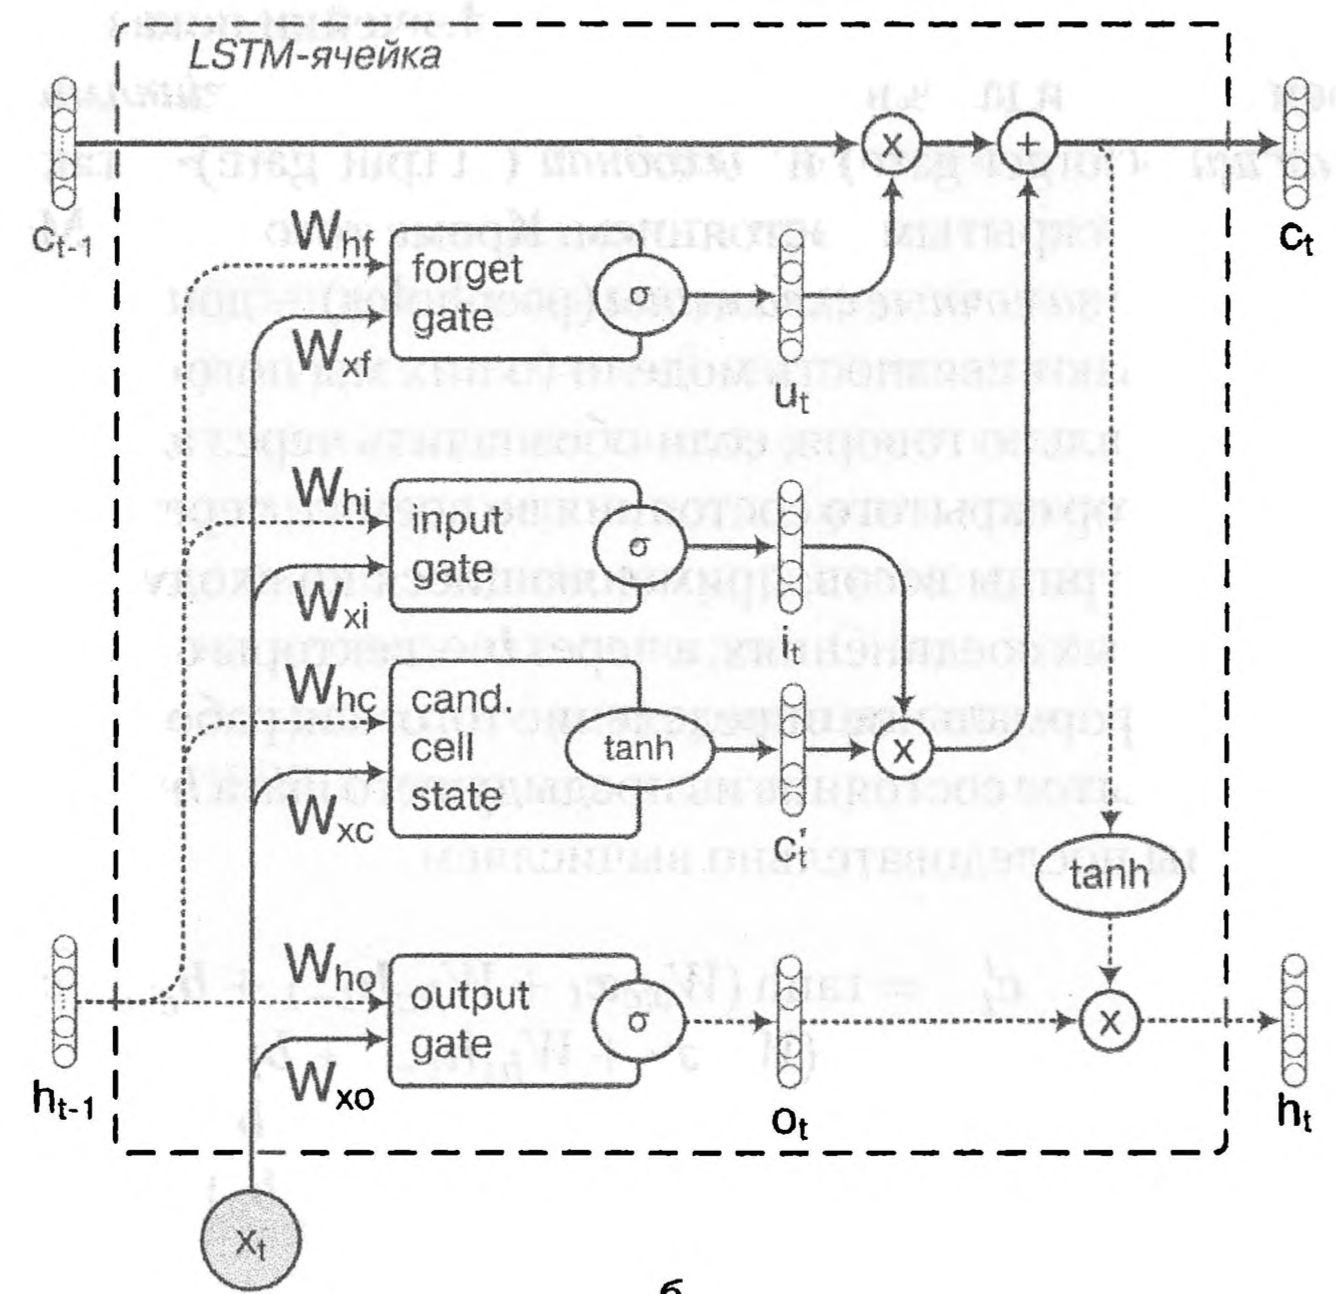
\includegraphics[width=0.8\textwidth]{lstm}
\caption{Ячейка LSTM. Источник: \cite{deeplearning}}
\label{fig:lstm}
\end{figure}

\subsubsection{Метод обратного распространения ошибки}
Метод обратного распространения ошибки -- одна из модификаций классического
градиентного спуска. Основная его идея состоит в распространении сигналов ошибки
от выходов сети к входам в направлении, обратном прямому распространению
сигнала. 